\documentclass[conference]{IEEEtran}
\IEEEoverridecommandlockouts
% The preceding line is only needed to identify funding in the first footnote. If that is unneeded, please comment it out.
\usepackage{cite}
\usepackage{amsmath,amssymb,amsfonts}
\usepackage{algorithmic}
\usepackage{graphicx}
\usepackage{textcomp}
\usepackage{xcolor}
\def\BibTeX{{\rm B\kern-.05em{\sc i\kern-.025em b}\kern-.08em
    T\kern-.1667em\lower.7ex\hbox{E}\kern-.125emX}}
\begin{document}

\title{ Security Issues in Cloud Computing 
}

\author{\IEEEauthorblockN{ Dr. Trevor M. Tomesh }
\IEEEauthorblockA{\textit{Dept. of Computer Science} \\
\textit{Lakehead University}\\
ttomesh@lakeheadu.ca }
\and
\IEEEauthorblockN{Kutala Mohan Prasad}
\IEEEauthorblockA{\textit{Lakehead University} \\
\textit{Student Id: 1154915}\\
mkutala@lakeheadu.ca}
}

\maketitle

\begin{abstract}

Cloud computing is a general term for anything that involves delivering hosted services over the internet.The name cloud computing was inspired by the cloud symbol that's often used to represent the internet in flowcharts and diagrams.Cloud infrastructure involves the hardware and software components required for proper implementation of a cloud computing model. Cloud computing works by allowing client devices to access data over the internet, from remote servers, databases and computers.Cloud computing offers an innovative business model for organizations to adopt IT services without upfront investment. Apart from popularity that gains by the cloud computing still some organisations are yet to move from physical to cloud platform hosting, that is due to the security. Customers need to be vigilant in understanding the risks of data breaches in this new environment. This paper introduces a detailed analysis of the cloud computing security issues and some vulnerabilities focusing on the cloud computing.

\end{abstract}

\section{Introduction}

Now a days most interesting topic and enhancement in internet world is Cloud Computing. As per my analysis I saw there is drastic change in Information technology and its capabilities. From small scale industries to large scale industries we see lot of movements from physical machines to cloud due to different reasons. Cloud computing is a set of services that provided by different IT vendors for rental to perform our activities in software era. Usually cloud computing services are delivered by a third party provider who owns the infrastructure. It advantages to mention but a few include scalability, resilience, flexibility, efficiency and outsourcing non-core activities. Cloud computing offers an innovative business model for organizations to adopt IT services without upfront investment. But as more and more information on individuals and companies are placed in the cloud, concerns are beginning to grow about just how safe an environment it is. Despite of all the hype surrounding the cloud, customers are still reluctant to deploy their business in the cloud. Customers must demand transparency, avoiding vendors that refuse to provide detailed information on security programs. Ask questions related to the qualifications of policy makers, architects, coders and operators, risk-control processes and technical mechanisms and the level of testing that's been done to verify that service and control processes are functioning as intended, and that vendors can identify unanticipated vulnerabilities. As per kuyoro Security is the most important role when compare to other services “Security issues in cloud computing has played a major role in slowing down its acceptance, in fact security ranked first as the greatest challenge issue of cloud computing” [3].


\section{SECURITY ISSUES IN CLOUD COMPUTING}

Vulnerability is an important factor of risk. Risk defines as “the potential that a given threat will exploit vulnerabilities of an asset or group of assets and thereby cause harm to the organization,” measuring it in terms of both the likelihood of an event and its consequence.

Cloud computing builds heavily on capabilities available through several core technologies

Security of the cloud computing will mostly depend upon the services which were provided by the cloud vendors as per my analysis and referred papers below I see only three main services in all cloud vendors as shown in Figure 1.

\subsection{Infrastructure as a Service (IaaS)}
Infrastructure as a Service is a single tenant cloud layer where the Cloud computing vendor’s dedicated resources are only shared with contracted clients at a pay-per-use fee. This greatly minimizes the need for huge initial investment in computing hardware such as servers, networking devices and processing power. They also allow varying degrees of financial and functional flexibility not found in internal data centers or with collocation services, because computing resources can be added or released much more quickly and cost-effectively than in an internal data center or with a collocation service [2]. IaaS and other associated services have enabled startups and other businesses focus on their core competencies without worrying much about the provisioning and management of infrastructure. IaaS completely abstracted the hardware beneath it and allowed users to consume infrastructure as a service without bothering anything about the underlying complexities. The cloud has a compelling value proposition in terms of cost, but ‘out of the box’ IaaS only provides basic security (perimeter firewall, load balancing, etc.) and applications moving into the cloud will need higher levels of security provided at the host. For infrastructure as a service (IaaS) offerings, administrators typically implement associated services and APIs, such as the management access for customers, using Web ap¬plication/service technologies.

\begin{figure}[ht!] %!t
\centering
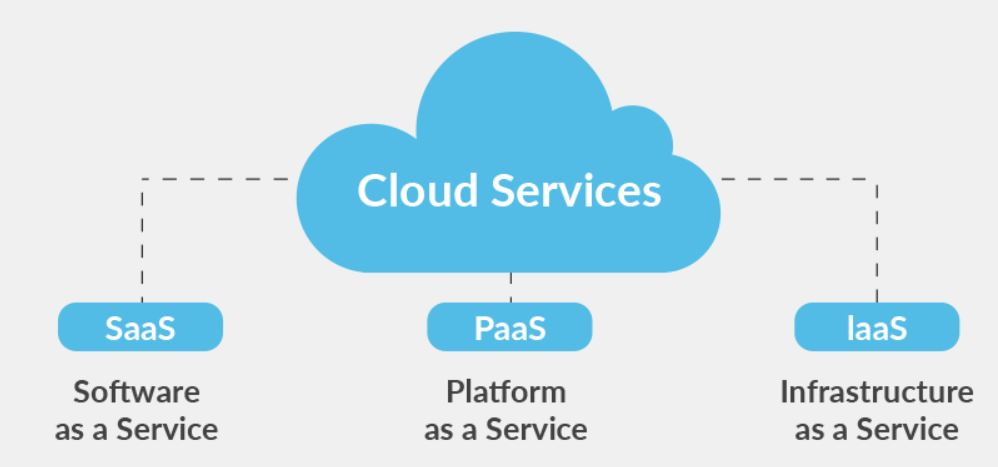
\includegraphics[width=3.5in]{Services-Fig2.JPG}
\caption{Services in Cloud Computing}
\label{Courant_2}
\end{figure}

\subsection{Software as a Service (SaaS)}
Software-as-a-Service, or SaaS for short, is a cloud-based method of providing software to users. SaaS users subscribe to an application rather than purchasing it once and installing it. Users can log into and use a SaaS application from any compatible device over the Internet. The actual application runs in cloud servers that may be far removed from a user's location. SaaS is most often implemented to provide business software functionality to enterprise customers at a low cost while allowing those customers to obtain the same benefits of commercially licensed, internally operated software without the associated complexity of installation, management, support, licensing, and high initial cost. The architecture of SaaS-based applications is specifically designed to support many concurrent users (multitenancy) at once. Software as a service applications are accessed using web browsers over the Internet therefore web browser security is vitally important. Information security officers will need to consider various methods of securing SaaS applications. Web Services (WS) security, Extendable Markup Language (XML) encryption, Secure Socket Layer (SSL) and available options which are used in enforcing data protection transmitted over the Internet.[4]
\subsection{Platform as a service (PaaS)}

Platform as a Service (PaaS) provides a runtime environment. It allows programmers to easily create, test, run, and deploy web applications. You can purchase these applications from a cloud service provider on a pay-as-per use basis and access them using the Internet connection. In PaaS, back end scalability is managed by the cloud service provider, so end- users do not need to worry about managing the infrastructure. PaaS includes infrastructure (servers, storage, and networking) and platform (middleware, development tools, database management systems, business intelligence, and more) to support the web application life cycle. For Example: Google App Engine, Force.com, Joyent, Azure. PaaS providers provide various programming languages for the developers to develop the applications. Some popular programming languages provided by PaaS providers are Java, PHP, Ruby, Perl, and Go. This offers an integrated set of developer environment that a developer can tap to build their applications without having any clue about what is going on underneath the service. It offers developers a service that provides a complete software development life cycle management, from planning to design to building applications to deployment to testing to maintenance. Everything else is abstracted away from the “view” of the developers. Platform as a service cloud layer works like IaaS but it provides an additional level of ‘rented’ functionality. Clients using PaaS services transfer even more costs from capital investment to operational expenses but must acknowledge the additional constraints and possibly some degree of lock-in posed by the additional functionality layers [5]. The use of virtual machines act as a catalyst in the PaaS layer in Cloud computing. Virtual machines must be protected against malicious attacks such as cloud malware. Therefore maintaining the integrity of applications and well enforcing accurate authentication checks during the transfer of data across the entire networking channels is fundamental.

\subsection{Cryptography}
Many cloud computing security requirements are solvable only by using cryptographic techniques. Because cryptography is frequently used to
overcome storage-related vulnerabilities, this core
technology’s vulnerabilities insecure or obsolete
cryptography and poor key management play a special
role for cloud storage.

\section{Main Models in Cloud Computing}
As we know before storing our data or selecting the services in cloud computing we will see different types of cloud features or models in which they are offering for example who will access our data? Who will have read, write and modify access to it for these doubts each cloud vendor has given different types of models to deploy our data in major we have four type as shown in Figure 2.


\begin{figure}[ht!] %!t
\centering
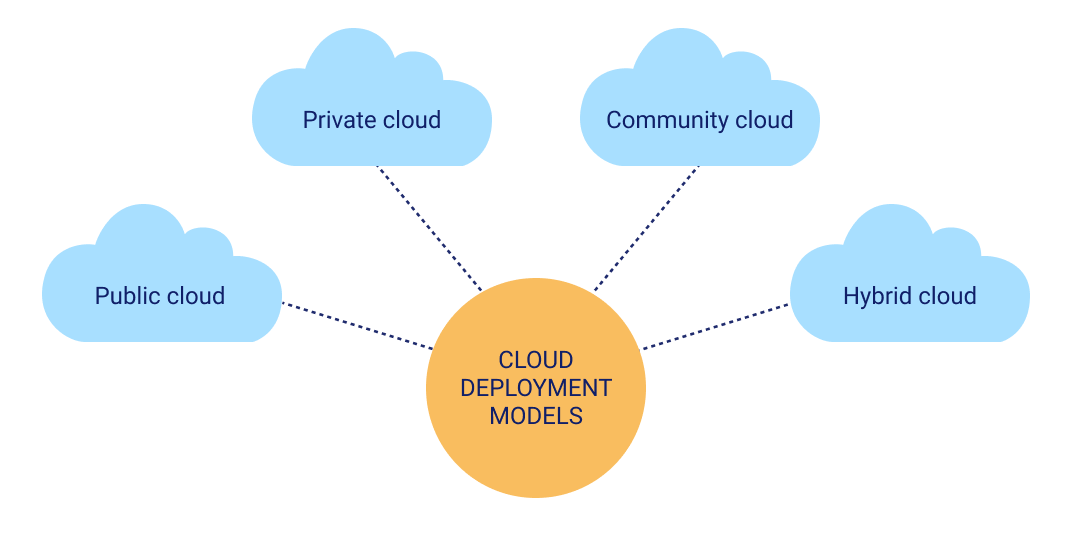
\includegraphics[width=3.5in]{Cloud-Deployment-Models_fig1.png}
\caption{Models in Cloud Computing}
\label{Courant_2}
\end{figure}

\subsection{Public cloud}
Public cloud is open to all to store and access information via the Internet using the pay-per-usage method.In public cloud, computing resources are managed and operated by the Cloud Service Provider (CSP).Example: Amazon elastic compute cloud (EC2), IBM SmartCloud Enterprise, Microsoft, Google App Engine, Windows Azure Services Platform. Public clouds are less secure than the other cloud models because it places an additional burden of ensuring all applications and data accessed on the public cloud are not subjected to malicious attacks.

\subsection{Private cloud}
Private cloud is also known as an internal cloud or corporate cloud. It is used by organizations to build and manage their own data centers internally or by the third party. It can be deployed using Opensource tools such as Openstack and Eucalyptus. Utilization on the private cloud can be much more secure than that of the public cloud because of its specified internal exposure. Only the organization and designated stakeholders may have access to operate on a specific Private cloud.

\subsection{Hybrid cloud}
Hybrid Cloud is a combination of the public cloud and the private cloud. Hybrid cloud is partially secure because the services which are running on the public cloud can be accessed by anyone, while the services which are running on a private cloud can be accessed only by the organization's users. It has a capability of combining virtual and physical, collocated assets for example, a mostly virtualized environment that requires physical servers, routers, or other hardware such as a network appliance acting as a firewall or spam filter.

\subsection{Community Cloud}
Community cloud is a cloud infrastructure that allows systems and services to be accessible by a group of several organizations to share the information. It is owned, managed, and operated by one or more organizations in the community, a third party, or a combination of them. For Example, Our government organization within India may share computing infrastructure in the cloud to manage data.

\section{Security Risks of Cloud Computing}
Some most common Security Risks of Cloud Computing are given below

\subsection{Data Loss}
Data loss is the most common cloud security risks of cloud computing. It is also known as data leakage. Data loss is the process in which data is being deleted, corrupted, and unreadable by a user, software, or application. In a cloud computing environment, data loss occurs when our sensitive data is somebody else's hands, one or more data elements can not be utilized by the data owner, hard disk is not working properly, and software is not updated.

\subsection{Data Breach}
Data Breach is the process in which the confidential data is viewed, accessed, or stolen by the third party without any authorization, so organization's data is hacked by the hackers.

\subsection{Denial of Service (DoS) attacks}
Denial of service (DoS) attacks occur when the system receives too much traffic to buffer the server. Mostly, DoS attackers target web servers of large organizations such as banking sectors, media companies, and government organizations. To recover the lost data, DoS attackers charge a great deal of time and money to handle the data.

\subsection{Account hijacking}
Account hijacking is a serious security risk in cloud computing. It is the process in which individual user's or organization's cloud account (bank account, e-mail account, and social media account) is stolen by hackers. The hackers use the stolen account to perform unauthorized activities.

Web application technologies must overcome the problem that, by design, the HTTP protocol is a stateless protocol, whereas Web applications require some notion of session state. Many techniques implement session handling and as any security professional knowledgeable in Web application security
will testify many session handling implementations are vulnerable to session riding and session hijacking. Whether session riding/hijacking vulnerabilities are intrinsic to Web application technologies or are
only prevalent in many current implementations is arguable in any case, such vulnerabilities are certainly relevant for cloud computing.

\subsection{Investigation support}
Investigating inappropriate or illegal activity may be impossible in cloud computing, Gartner warns. "Cloud services are especially difficult to investigate, because logging and data for multiple customers may be co-located and may also be spread across an ever-changing set of hosts and data centers. If you cannot get a contractual commitment to support specific forms of investigation, along with evidence that the vendor has already successfully supported such activities, then your only safe assumption is that investigation and discovery requests will be impossible."[1]

\section{Conclusion}
Cloud computing has started new era in the internet world not only for data storage but also on the availability, Security and maintenance. However we need to understand the security issues or any challenges among all cloud based technologies before committing the code or data in third party. In this paper I have concentrated major security issues in different models and services. In future I will concentrate more on issues and Vulnerabilities in the cloud computing sector. 

\begin{thebibliography}{00}
\bibitem{b1} B. Grobauer, T. Walloschek and E. Stöcker, "Understanding Cloud Computing
Vulnerabilities," IEEE Security and Privacy, vol. 99, 2010.


\bibitem{b2} J. Brodkin. (2008, Jun.). “Gartner: Seven cloud-computing security risks.” Infoworld,
Available: <http://www.infoworld.com/d/security-central/gartner-seven-cloudcomputingsecurity-
risks-853?page=0,1> [Mar. 13, 2009].


\bibitem{b3} SO Kuyoro, F Ibikunle, O Awodele  “Cloud computing security issues and challenges”

\bibitem{b4} S. Subashini, and V. Kavitha. (2010) “A survey on security issues in service delivery
models of cloud computing.” J Network Comput Appl doi:10.1016/j.jnca.2010.07.006. Jul.,
2010.

\bibitem{b5} Global Netoptex Incorporated. “Demystifying the cloud. Important opportunities, crucial
choices.” pp4-14. Available: http://www.gni.com [Dec. 13, 2009].

\bibitem{b6} S. Arnold (2009, Jul.). “Cloud computing and the issue of privacy.” KM World, pp14-22.
Available: www.kmworld.com [Aug. 19, 2009].

\end{thebibliography}

\end{document}